\documentclass[conference]{IEEEtran}
\IEEEoverridecommandlockouts

% =========================================================================
% PACKAGES
% =========================================================================
\usepackage{cite}
\usepackage{amsmath,amssymb,amsfonts,amsthm}
\usepackage{graphicx}
\usepackage{textcomp}
\usepackage{xcolor}
\usepackage{booktabs}
\usepackage{array}
\usepackage{enumitem}
\usepackage{microtype}
\usepackage{url}

% Mathematical environments
\newtheorem{theorem}{Theorem}
\newtheorem{lemma}{Lemma}
\newtheorem{definition}{Definition}

% Compact lists for two-column layout
\setlist{nosep,leftmargin=*,labelsep=0.5em}

% Unit shortcuts
\newcommand{\degC}{^{\circ}\mathrm{C}}
\newcommand{\Wm}{\mathrm{W/m^2}}

\def\BibTeX{{\rm B\kern-.05em{\sc i\kern-.025em b}\kern-.08em
    T\kern-.1667em\lower.7ex\hbox{E}\kern-.125emX}}

\begin{document}

% =========================================================================
% TITLE AND AUTHORS
% =========================================================================
\title{Solaraeus: A Physics-Based 3D Urban Microclimate Digital Twin with Certified Incremental Radiative Transfer, GPU Acceleration, and an AI Solver for Optimal Intervention Placement\thanks{This research is developed under the Solaraeus Open Urban Microclimate Initiative. Source code, reproducible verification suites, and interactive viewer assets are maintained at \texttt{https://github.com/ayushsingh08-ds/solaraeus}.}}

\author{
\IEEEauthorblockN{Ayush Singh}
\IEEEauthorblockA{\textit{Department of Computational Science} \\
\textit{and Engineering (Data Science)} \\
\textit{Dayananda Sagar University}\\
Bengaluru, Karnataka, India \\
eng23ds0098@gmail.com}
\and
\IEEEauthorblockN{Dr. Jobin Thomas}
\IEEEauthorblockA{\textit{Department of Computational Science} \\
\textit{and Engineering (Data Science)} \\
\textit{Dayananda Sagar University}\\
Bengaluru, Karnataka, India \\
jobinthomas-ds@dsu.edu.in}
}

\maketitle

% =========================================================================
% ABSTRACT
% =========================================================================
\begin{abstract}
Pedestrian thermal stress poses an escalating public health crisis in rapidly densifying tropical metropolises, yet existing microclimate modeling packages operate as monolithic, desktop-bound batch solvers. When localized architectural interventions (e.g., shade canopies or tree plantings) are evaluated, traditional engines discard domain state and recompute all spatial fields from scratch, creating a computational bottleneck that precludes real-time interactive design and automated optimization. Furthermore, existing tools lack an automated \textbf{AI Solver} capable of discovering optimal spatial placements and orientations of cooling interventions across complex street canyons. In this paper, we present \textbf{Solaraeus}, an end-to-end, physics-based 3D urban microclimate digital twin, GPU computational engine, and AI placement solver. Solaraeus harmonizes open geospatial datasets---Overture building vector polygons, Google Open Buildings machine-learning height estimates, FABDEM topography, and NOAA/NASA POWER meteorological fluxes---into an automated Python and CUDA C++ simulation pipeline. The core engine executes astronomical solar vector tracking, Steyn (1980) Sky View Factor (SVF) calculation across 36 azimuth radials, 3D Möller--Trumbore ray-traced directional shadows, 6-flux Stefan--Boltzmann Mean Radiant Temperature ($T_{\mathrm{mrt}}$) balance, and Universal Thermal Climate Index (UTCI) biometeorological stress evaluation. To overcome the recomputation bottleneck, we formulate and prove a \textit{Certified Incremental Solver} with closed-form error bounds $B_T(x) \le \varepsilon_T = 0.50\,\mathrm{K}$ grounded in concave Stefan--Boltzmann linearization and solid-angle horizon truncation decay, coupled with a resident-memory CUDA GPU acceleration engine on NVIDIA RTX 4050. Built upon this certified foundation, we introduce an active learning \textbf{AI Solver for Optimal Intervention Placement} driven by multi-target decision-tree ensembles (Random Forest / Extra-Trees), a 20-dimensional permutation-invariant feature embedding, a geometric feasibility classifier, and Upper Confidence Bound (UCB) acquisition to autonomously discover Pareto-optimal shade canopy configurations.

Solaraeus is evaluated on an empirical real-world digital twin of the Church Street pedestrian corridor in Bengaluru, India ($380\,\mathrm{m} \times 296\,\mathrm{m}$ simulation domain, $2.0\,\mathrm{m}$ grid, $28{,}120$ cells, 123 buildings). Baseline simulations reveal severe pedestrian heat stress during peak pre-monsoon conditions ($T_a = 35.0\degC$, $\mathrm{GHI} = 755.97\,\Wm$), with corridor $T_{\mathrm{mrt}}$ averaging $45.81\degC$ and UTCI averaging $36.49\degC$ (Strong Heat Stress), contrasting against building-shaded zones by $\Delta T_{\mathrm{mrt}} = 11.89\,\mathrm{K}$. Introducing an overhead shade canopy ($\mathrm{BLR\_SHADE\_001}$, $6\,\mathrm{m} \times 3\,\mathrm{m}$) delivers a peak localized cooling relief of $-12.62\,\mathrm{K}$ $T_{\mathrm{mrt}}$ and $-3.10\,\mathrm{K}$ UTCI. The certified incremental solver recomputes only $72$ cells ($0.26\%$) while reusing $28{,}048$ cells ($99.74\%$), avoiding $925{,}584$ rays ($99.74\%$ work reduction) with a maximum observed domain error of $0.0289\,\mathrm{K} \ll 0.50\,\mathrm{K}$ and zero certificate violations across 18 audited criteria. On an NVIDIA RTX 4050 GPU, the resident incremental kernel executes in $11.40\,\mathrm{ms}$ ($500.87\times$ speedup over full CPU recomputation; $36.84\times$ over CPU incremental). Guided by these certified evaluations, our AI Solver evaluates over $4{,}400$ candidate proposals and identifies an optimal dual-canopy configuration ($\mathrm{CAND\_4196\_SURR}$, $22.87\,\mathrm{m}^2$) delivering $12.68\,\mathrm{K}$ peak cooling with zero spatial shadow overlap, while achieving an active learning advantage over random search baselines. Outputs are serialized into typed JSON contracts and ingested by an interactive Three.js 3D WebGL digital twin with custom GLSL thermal shaders.
\end{abstract}

\begin{IEEEkeywords}
Urban microclimate, mean radiant temperature, UTCI, certified incremental computation, GPU acceleration, CUDA, AI solver, machine learning, surrogate optimization, digital twin, Bengaluru, thermal comfort.
\end{IEEEkeywords}

% =========================================================================
% SECTION I: INTRODUCTION
% =========================================================================
\section{Introduction}

Accelerating global urbanization compounded by climate-induced heatwaves has intensified the Urban Heat Island (UHI) effect, subjecting metropolitan populations to dangerous levels of outdoor physiological strain \cite{oke1982canyon,grimmond2010climate}. In dense tropical and equatorial cities such as Bengaluru, India ($12.97^\circ\,\mathrm{N}$), high solar elevation angles and narrow concrete-and-asphalt street canyons generate acute diurnal thermal loads. Within pedestrian corridors, outdoor thermal comfort during daylight hours is governed predominantly by the Mean Radiant Temperature ($T_{\mathrm{mrt}}$) rather than dry-bulb ambient air temperature ($T_a$) alone \cite{matzarakis2007modelling}. $T_{\mathrm{mrt}}$ integrates shortwave solar irradiance (direct beam, diffuse sky, and surface reflections) and longwave emissions from heated building facades and ground pavements incident upon the human body. Under direct tropical sun, radiant heat flux elevates pedestrian physiological sensation into the \textit{Strong} and \textit{Very Strong Heat Stress} classifications of the Universal Thermal Climate Index (UTCI) \cite{jendritzky2012universal,brode2012deriving}, inducing heat exhaustion and cardiovascular stress. Consequently, municipal urban planners, landscape architects, and municipal engineers urgently require high-resolution microclimatic models to evaluate localized heat mitigation interventions, such as overhead shade structures and tree plantings \cite{chen2012gis,chatzipoulka2016sky}.

To model urban outdoor microclimates, established software packages have been developed across distinct computational paradigms. Microscale Computational Fluid Dynamics (CFD) suites such as ENVI-met \cite{bruse1998simulating} simulate coupled atmospheric turbulence, convective transport, and vegetative biology; however, their prohibitive computational overhead---often requiring hours to days of CPU processing for a single diurnal cycle---precludes iterative design exploration. Conversely, decoupled radiation models such as the Solar and Longwave Environmental Irradiance Geometry (SOLWEIG) model within the Urban Multi-scale Environmental Predictor (UMEP) \cite{lindberg2008solweig,lindberg2018urban}, RayMan \cite{matzarakis2007modelling}, and Ladybug Tools \cite{sadeghipour2013ladybug} establish an efficient compromise by isolating 3D geometric radiative transfer from turbulent fluid flow. Because convective heat exchange accounts for less than one-third of pedestrian daytime thermal sensation in clear-sky conditions compared to radiation \cite{matzarakis2007modelling}, SOLWEIG models multi-directional shortwave and longwave fluxes on cylindrical human geometry by marching discrete rays across Digital Elevation Models (DEMs) to evaluate Sky View Factors (SVF) and cast shadows in seconds rather than hours \cite{gal2009sky,lindberg2010spatial}.

Despite their theoretical maturity, current microclimate modeling workflows suffer from four fundamental computational and operational bottlenecks. First, existing solvers operate as monolithic batch programs: whenever an urban designer introduces a localized architectural alteration---such as placing an overhead awning or planting a shade tree---the engine discards the entire domain and recalculates all grid cells from scratch, creating an acute computational bottleneck. Second, while heuristic spatial clipping can restrict updates, existing tools lack a mathematically certified, closed-form error bound guaranteeing that untouched cells do not exceed an acceptable thermal tolerance ($|\widetilde{T}_{\mathrm{mrt}}(x) - T_{\mathrm{mrt}}^{\mathrm{full}}(x)| \le \varepsilon_T$). Third, existing software lacks an automated \textbf{AI Solver} for optimal intervention placement: urban planners are left to rely on slow, manual trial-and-error placement because the multi-parameter combinatorial search space of 3D canopy coordinates, dimensions, orientations, and mutual clearance constraints cannot be practically traversed by brute-force simulations. Fourth, existing software remains desktop-bound, CPU-constrained, and disconnected from modern hardware-accelerated graphics pipelines, exporting static GIS rasters rather than publishing open, typed data contracts to interactive 3D WebGL digital twins.

To overcome these barriers, this paper presents \textbf{Solaraeus}, an end-to-end, physics-based 3D urban microclimate digital twin, GPU computational engine, and AI placement solver evaluated on an empirical pedestrian corridor in Church Street, Bengaluru, India ($380\,\mathrm{m} \times 296\,\mathrm{m}$ domain, $28{,}120$ cells, 123 buildings). This work addresses four core objectives: (1) automating geospatial harmonization of open building vectors, machine-learning height estimates, and atmospheric reanalysis into watertight 3D meshes; (2) formulating and proving a \textit{Certified Incremental Solver} that bounds approximation errors ($B_T(x) \le \varepsilon_T = 0.50\,\mathrm{K}$) via solid-angle horizon decay and concave Stefan--Boltzmann linearization, reusing over $99.7\%$ of static grid cells; (3) developing a resident-memory CUDA GPU acceleration engine on NVIDIA RTX 4050 executing incremental updates in $11.40\,\mathrm{ms}$ ($500.87\times$ speedup over full CPU recomputation); (4) implementing an active learning \textbf{AI Solver for Optimal Intervention Placement} combining multi-target decision-tree ensembles with Upper Confidence Bound (UCB) acquisition to autonomously search the 14-parameter non-convex canyon space; and (5) delivering an open, interactive Three.js 3D WebGL digital twin.

% =========================================================================
% SECTION II: LITERATURE REVIEW
% =========================================================================
\section{Literature Review}

\subsection{Outdoor Thermal Comfort and Mean Radiant Temperature}
Pedestrian thermal sensation in urban outdoor spaces has been extensively investigated \cite{oke1982canyon,grimmond2010climate}. Fanger's seminal work \cite{fanger1970thermal} established the fundamental heat exchange balance between the human body and the surrounding thermal environment. Outdoor biometeorological research subsequently formalized indices such as the Physiological Equivalent Temperature (PET) \cite{matzarakis2007modelling} and the Universal Thermal Climate Index (UTCI) \cite{jendritzky2012universal,brode2012deriving}. UTCI couples a multi-node dynamic human thermoregulation model (Fiala et al.\ \cite{fiala2012utci}) with an adaptive clothing insulation algorithm. Across diverse urban canyon morphologies, $T_{\mathrm{mrt}}$ represents the single most influential meteorological driver of outdoor heat stress: daytime fluctuations in shortwave solar and longwave terrestrial radiant fluxes impact pedestrian physiological strain more than twice as intensely as equivalent variations in ambient air temperature \cite{matzarakis2007modelling,brode2012deriving}.

\subsection{Radiative Transfer Modeling and SOLWEIG}
Simulating outdoor radiative transfer requires solving complex line-of-sight occlusions across 3D urban geometries \cite{robinson2004sun,krayenhoff2014multi}. A foundational metric is the Sky View Factor (SVF), defined as the ratio of visible radiant sky hemisphere unobstructed by surrounding built surfaces \cite{chen2012gis,chatzipoulka2016sky}. Steyn \cite{steyn1980svf} introduced the angular ray-marching method across radial azimuths over digital elevation grids. Lindberg et al.\ extended this concept in the SOLWEIG model \cite{lindberg2008solweig,lindberg2010spatial}, modeling direct beam, diffuse sky irradiance, and reflected longwave emissions across six cardinal orthogonal directions (upward, downward, north, south, east, and west) on Fanger's rotationally symmetric human cylinder. While SOLWEIG dramatically reduces runtime relative to Navier--Stokes CFD suites, its implementation in UMEP relies on raster-based Python/QGIS batch processing, where any spatial scene edit requires recomputing the entire raster domain \cite{lindberg2018urban}.

\subsection{GPU Ray Tracing and Incremental Spatial Computation}
In computer graphics and computational geometry, hardware-accelerated ray tracing and spatial caching (e.g., Bounding Volume Hierarchies, shadow map caching, and temporal reprojection) are standard techniques for avoiding redundant work across interactive updates \cite{wald2014embree,parker2010optix}. In urban environmental simulation, researchers have explored GPU acceleration to speed up solar irradiance calculations \cite{bauer2020accelerating,zhang2019gpu,kastner2020ray}. However, existing GPU implementations remain strictly batch-oriented: when a localized geometric intervention (e.g., shade canopy or tree) is modified, the solver recomputes the entire scene from scratch. While incremental visibility techniques have been studied conceptually in spatial computing \cite{teller1992visibility}, their rigorous mathematical coupling with certified thermal error bounds and multi-directional SOLWEIG-compatible flux integration has not been realized in urban microclimate science.

\subsection{AI and Machine Learning Solvers for Urban Spatial Optimization}
Optimizing microclimatic interventions across complex urban canyons is intrinsically challenging due to non-convex physical objective landscapes, geometric canyon boundaries, and significant simulation latency \cite{forrester2008engineering}. Traditional urban design workflows rely on heuristic manual placement or brute-force grid searches that scale poorly to multi-parameter spaces. To overcome this, surrogate-assisted optimization and active machine learning solvers replace computationally expensive numerical evaluations with statistical learning models (e.g., Gaussian processes, radial basis functions, and decision-tree ensembles) guided by exploration-exploitation acquisition policies \cite{forrester2008engineering}. While Gaussian processes suffer from $\mathcal{O}(N^3)$ kernel inversion bottlenecks in high-dimensional tabular spaces, ensemble tree architectures (such as Random Forests and Extra-Trees) provide robust variance estimates and scale efficiently to multi-target physical predictions. Coupling certified GPU-accelerated microclimate engines with active machine learning solvers enables automated, physically sound discovery of Pareto-optimal urban interventions.

% =========================================================================
% SECTION III: DESCRIPTION OF DATA
% =========================================================================
\section{Description of Data}

\subsection{Church Street, Bengaluru Study Site and Domain Boundary}
To evaluate Solaraeus on an authentic, high-density tropical urban corridor, we selected Church Street in central Bengaluru (Karnataka, India; $12.974900^\circ\,\mathrm{N}$, $77.605400^\circ\,\mathrm{E}$). Church Street is a flagship pedestrian-priority commercial avenue characterized by continuous multi-story retail and office facades, dense foot traffic, and limited natural tree shade. During the pre-monsoon summer season (March to May), Bengaluru experiences acute daytime heat with clear-sky solar irradiances exceeding $750\,\Wm$ and ambient temperatures surpassing $35^\circ\mathrm{C}$, creating severe pedestrian heat stress.

The simulation domain is partitioned into:
\begin{itemize}
    \item \textbf{Core Study Block:} A $218.46\,\mathrm{m} \times 135.05\,\mathrm{m}$ bounding area ($28{,}840.88\,\mathrm{m}^2$) enclosing 37 mapped core building footprints along the primary pedestrian promenade.
    \item \textbf{Shadow Context Domain:} The core site expanded outward by a $75\,\mathrm{m}$ metric buffer to capture incoming building shadow rays cast by external high-rises at oblique solar angles. The resulting domain measures $380.0\,\mathrm{m} \times 296.0\,\mathrm{m}$, discretized onto a uniform $2.0\,\mathrm{m}$ grid ($190 \times 148 = 28{,}120$ cells).
    \item \textbf{Pedestrian Corridor:} A 12-metre-wide corridor centered along Church Street containing $N = 668$ active pedestrian ground cells reserved for detailed comfort auditing.
\end{itemize}

Geospatial layers are harmonized into Universal Transverse Mercator (UTM) Zone 43N (EPSG:32643, WGS~84 datum). The local simulation coordinate origin $(0, 0)$ is pinned to $X_{\mathrm{origin}} = 782{,}541.81\,\mathrm{m}\,\mathrm{E}, Y_{\mathrm{origin}} = 1{,}435{,}736.11\,\mathrm{m}\,\mathrm{N}$. Because the street corridor is oriented obliquely to True North, the local grid convergence angle is strictly computed as $\gamma = +0.5854^\circ$. All solar azimuth calculations are rotated by $\gamma$ to align true astronomical vectors with metric grid axes without spatial distortion.

\subsection{Dual-Taxonomy Building Mesh Data}
Building structural envelopes are synthesized using a dual-taxonomy dataset reconciling open Overture Maps vector polygons with Google Open Buildings machine-learning footprints. The scene integrates 123 buildings (37 core, 86 context). Building heights are categorized into direct height records for 7 municipal structures ($H_k \in [8.0\,\mathrm{m}, 35.0\,\mathrm{m}]$) and machine-learning inferred heights for 116 buildings derived from Google Open Buildings confidence rasters ($H_k \in [6.5\,\mathrm{m}, 28.0\,\mathrm{m}]$). All footprints are triangulated into watertight 3D meshes consisting of $2{,}136$ triangles with validated 2-manifold topology.

\subsection{Atmospheric and Solar Forcing Baseline}
Atmospheric forcing conditions were acquired for the extreme pre-monsoon heatwave of April 15, 2024 at 09:00 UTC (14:30 Indian Standard Time, IST). Boundary meteorology is derived from the NOAA Integrated Surface Database (ISD) Bengaluru City Station 43295099999 ($2.56\,\mathrm{km}$ southwest of Church Street): $T_a = 35.0\degC$, relative humidity $\mathrm{RH} = 19.73\%$, and pedestrian wind speed $v_{1.1} = 1.1\,\mathrm{m/s}$. Solar fluxes from NASA POWER satellite reanalysis provide $\mathrm{GHI} = 755.97\,\Wm$, $\mathrm{DNI} = 728.31\,\Wm$, and $\mathrm{DHI} = 172.18\,\Wm$. NOAA astronomical solar position algorithms evaluate the sun position at altitude $\alpha_s = 57.9160^\circ$ and Grid North azimuth $\phi_{\mathrm{grid}} = 267.5802^\circ$. Surface properties are set to building wall albedo $\alpha_{\mathrm{bldg}} = 0.20$, ground asphalt albedo $\alpha_{\mathrm{gnd}} = 0.15$, and building emissivity $\varepsilon_{\mathrm{bldg}} = 0.90$ (Table~\ref{tab:inputs}).

\begin{table}[!t]
\caption{Church Street Digital Twin Environmental Parameters}
\label{tab:inputs}
\centering
\renewcommand{\arraystretch}{1.12}
\setlength{\tabcolsep}{4pt}
\resizebox{\columnwidth}{!}{%
\begin{tabular}{@{}llcc@{}}
\toprule
\textbf{Parameter} & \textbf{Symbol} & \textbf{Value} & \textbf{Unit} \\
\midrule
Coordinate Projection & CRS & UTM Zone 43N & EPSG:32643 \\
Grid Convergence & $\gamma$ & $+0.5854$ & $\mathrm{deg}$ \\
Simulation Domain & $\Omega$ & $380 \times 296$ & $\mathrm{m}$ \\
Grid Resolution & $\Delta x, \Delta y$ & $2.0 \times 2.0$ & $\mathrm{m}$ \\
Active Grid Cells & $N_{\mathrm{grid}}$ & $28{,}120$ & cells \\
Total Buildings & $N_{\mathrm{bldg}}$ & 123 & structures \\
Watertight Triangles & $N_{\mathrm{tri}}$ & $2{,}136$ & triangles \\
Solar Altitude & $\alpha_s$ & $57.9160$ & $\mathrm{deg}$ \\
Solar Azimuth (Grid) & $\phi_{\mathrm{grid}}$ & $267.5802$ & $\mathrm{deg}$ \\
Air Temperature & $T_a$ & $35.0$ & $\degC$ \\
Relative Humidity & $\mathrm{RH}$ & $19.73$ & $\%$ \\
Pedestrian Wind Speed & $v_{1.1}$ & $1.1$ & $\mathrm{m/s}$ \\
Global Irradiance & $\mathrm{GHI}$ & $755.97$ & $\Wm$ \\
Direct Normal Irradiance & $\mathrm{DNI}$ & $728.31$ & $\Wm$ \\
Diffuse Irradiance & $\mathrm{DHI}$ & $172.18$ & $\Wm$ \\
\bottomrule
\end{tabular}%
}
\end{table}

\subsection{Topographic and Vegetation Priors}
Ground terrain is modeled at flat datum $z = 0.0\,\mathrm{m}$ for primary benchmarks, with synthetic and FABDEM topographic profiles evaluated under documented protocols. Street vegetation integrates 14 municipal tree census trees from the Bruhat Bengaluru Mahanagara Palike (BBMP) cataloged along the corridor, parameterized as Level~1 cylinder trunks and ellipsoid crowns with Beer--Lambert shortwave attenuation priors.

% =========================================================================
% SECTION IV: METHODOLOGY
% =========================================================================
\section{Methodology}

\subsection{System Architecture and Pipeline Overview}
The complete system architecture of Solaraeus is illustrated in Fig.~\ref{fig:arch}. The computational pipeline couples four modular stages: (1) geospatial data ingestion, (2) physics preprocessing and watertight 3D meshing, (3) dual-backend radiative transfer solvers (CPU and CUDA GPU), and (4) data contract export to an interactive 3D WebGL digital twin.

\begin{figure}[!t]
\centering
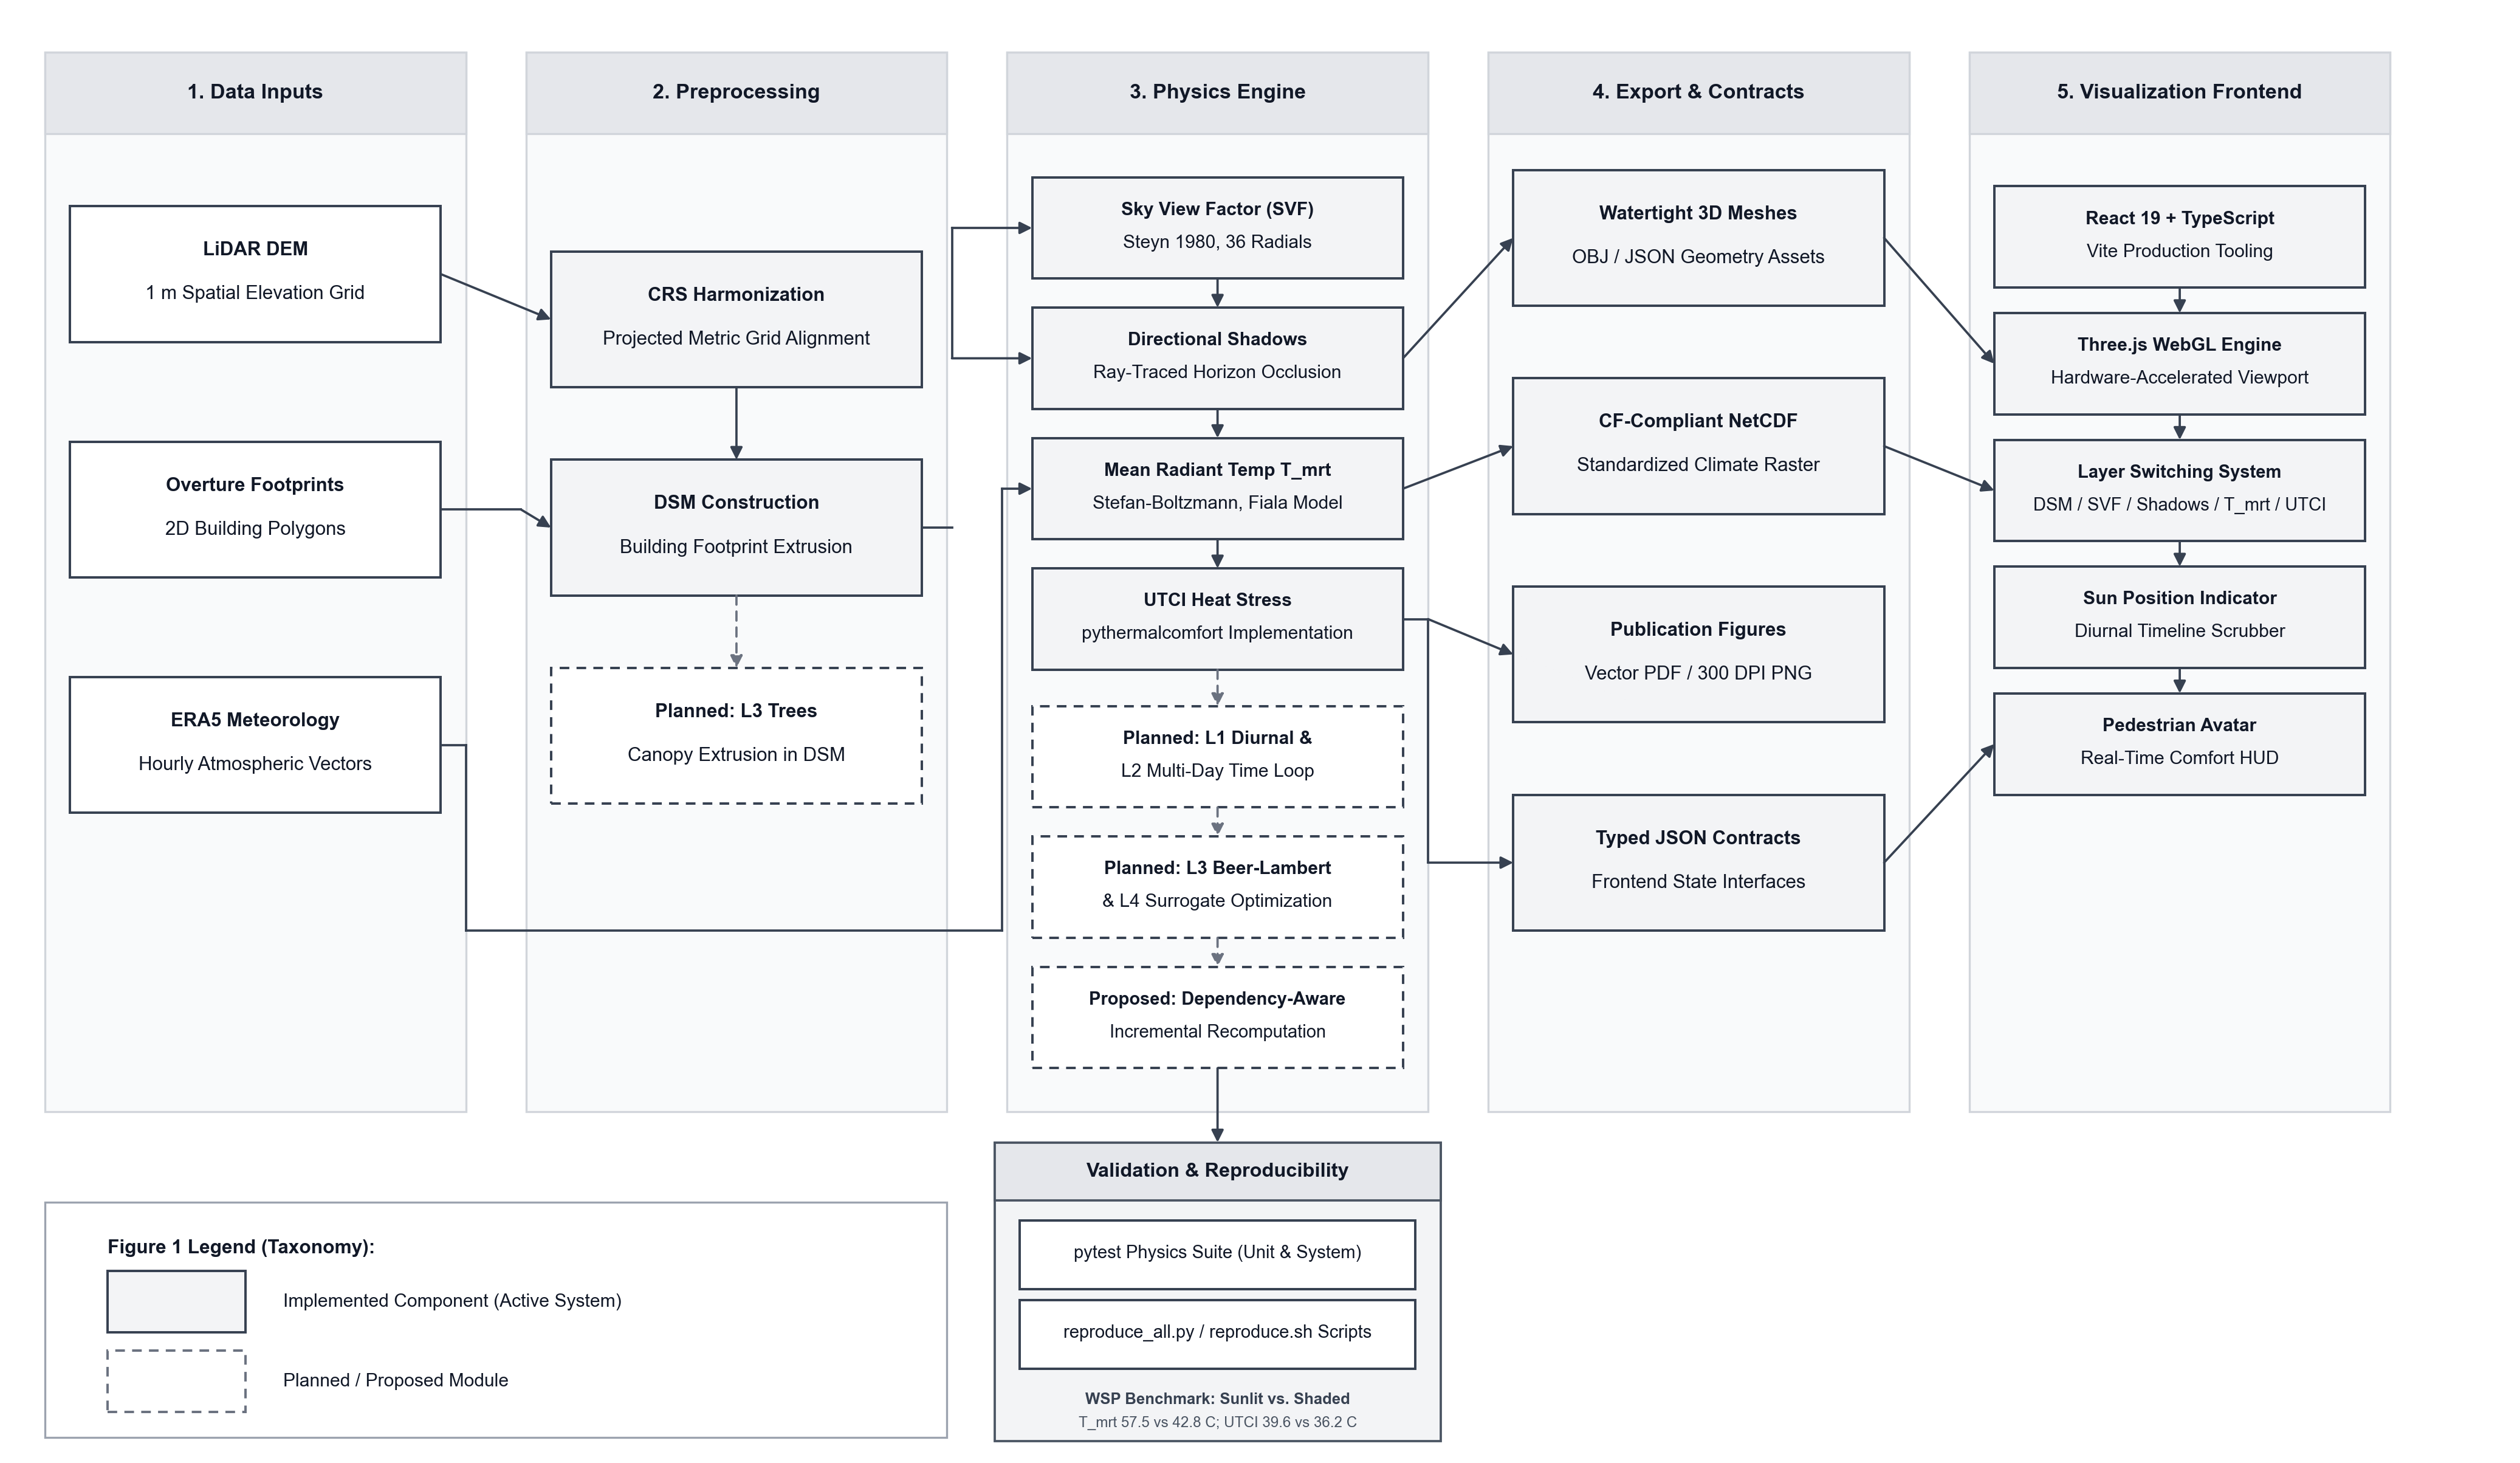
\includegraphics[width=\columnwidth]{fig1_architecture.png}
\caption{Solaraeus modular system architecture. Four cohesive layers link geospatial data ingestion, automated mesh preprocessing, dual-backend radiative solvers, and the interactive 3D WebGL digital twin.}
\label{fig:arch}
\end{figure}

\subsection{3D Radiative Transfer and Biometeorological Physics Formulation}
Sky View Factor $\Psi_{\mathrm{svf}}(u,v) \in [0, 1]$ at pedestrian eye level ($z_{\mathrm{ped}} = 1.1\,\mathrm{m}$) is calculated via the Steyn \cite{steyn1980svf} angular ray-marching formulation across $N_\phi = 36$ azimuth radials ($\Delta \phi = 10^\circ$, $R_{\max} = 150\,\mathrm{m}$):
\begin{equation}
    \Psi_{\mathrm{svf}}(u,v) = \frac{1}{N_{\phi}} \sum_{j=1}^{N_{\phi}} \bigl( 1 - \sin \beta(u,v,\phi_j) \bigr),
    \label{eq:svf_steyn}
\end{equation}
where $\tan \beta(u,v,\phi_j) = \max_{r \in (0, R_{\max}]} \frac{z_{\mathrm{mesh}}(u_r, v_r) - z_{\mathrm{ped}}}{r}$.

Ground-level shadow occlusions are resolved by casting directional rays toward unit sun vector $\vec{s}$ using the double-precision Möller--Trumbore ray-triangle intersection algorithm \cite{moller1997fast}:
\begin{equation}
    \begin{bmatrix} t \\ u_b \\ v_b \end{bmatrix} = \frac{1}{\vec{P} \cdot \vec{E}_1} \begin{bmatrix} \vec{Q} \cdot \vec{E}_2 \\ \vec{P} \cdot \vec{T} \\ \vec{Q} \cdot \vec{D} \end{bmatrix},
    \label{eq:moller_trumbore}
\end{equation}
yielding binary shadow mask $\mathcal{S}(u,v) \in \{0, 1\}$.

Total radiant energy absorbed by a pedestrian is evaluated across six orthogonal spatial directions on Fanger's cylindrical human geometry \cite{fanger1970thermal,lindberg2008solweig}:
\begin{equation}
    \Phi_{\mathrm{tot}}(u,v) = \alpha_p \sum_{i=1}^6 F_i K_i(u,v) + \varepsilon_p \sum_{i=1}^6 F_i L_i(u,v),
    \label{eq:flux_sum}
\end{equation}
where $\alpha_p = 0.70$, $\varepsilon_p = 0.97$, $F_{\mathrm{up}} = F_{\mathrm{down}} = 0.06$, and $F_{\mathrm{sides}} = 0.22$. Shortwave fluxes combine $K_{\mathrm{dir}} = I_{\mathrm{dir}} \mathcal{S}$, $K_{\mathrm{diff}} = I_{\mathrm{diff}} \Psi_{\mathrm{svf}}$, and reflected terms $K_{\mathrm{refl}} = (1 - \Psi_{\mathrm{svf}})\alpha_{\mathrm{bldg}} I_{\mathrm{glob}} + \alpha_{\mathrm{gnd}} I_{\mathrm{glob}}$. Longwave fluxes resolve $L_{\mathrm{down}} = \Psi_{\mathrm{svf}} L_{\mathrm{sky}} + (1 - \Psi_{\mathrm{svf}}) \varepsilon_{\mathrm{bldg}} \sigma T_{\mathrm{bldg}}^4$.

Mean Radiant Temperature ($T_{\mathrm{mrt}}$ in Kelvin) is obtained via Stefan--Boltzmann inversion:
\begin{equation}
    T_{\mathrm{mrt}}(u,v) = \left( \frac{\Phi_{\mathrm{tot}}(u,v)}{\sigma} \right)^{1/4},
    \label{eq:tmrt}
\end{equation}
with $\sigma = 5.67037 \times 10^{-8}\,\mathrm{W/(m^2\,K^4)}$. UTCI is computed via the operational 6th-order polynomial $f_{\mathrm{poly}}(T_a, T_{\mathrm{mrt}}, v_{1.1}, \mathrm{RH})$ from \texttt{pythermalcomfort}.

\subsection{Certified Incremental Radiative Transfer}
When an urban canopy intervention $\mathcal{P}$ is introduced, Solaraeus partitions the domain into recomputed dirty cells $\Omega_{\mathrm{dirty}}$ and invariant clean cells $\Omega_{\mathrm{clean}} = \Omega \setminus \Omega_{\mathrm{dirty}}$ (Fig.~\ref{fig:incremental}).

\begin{figure}[!t]
\centering
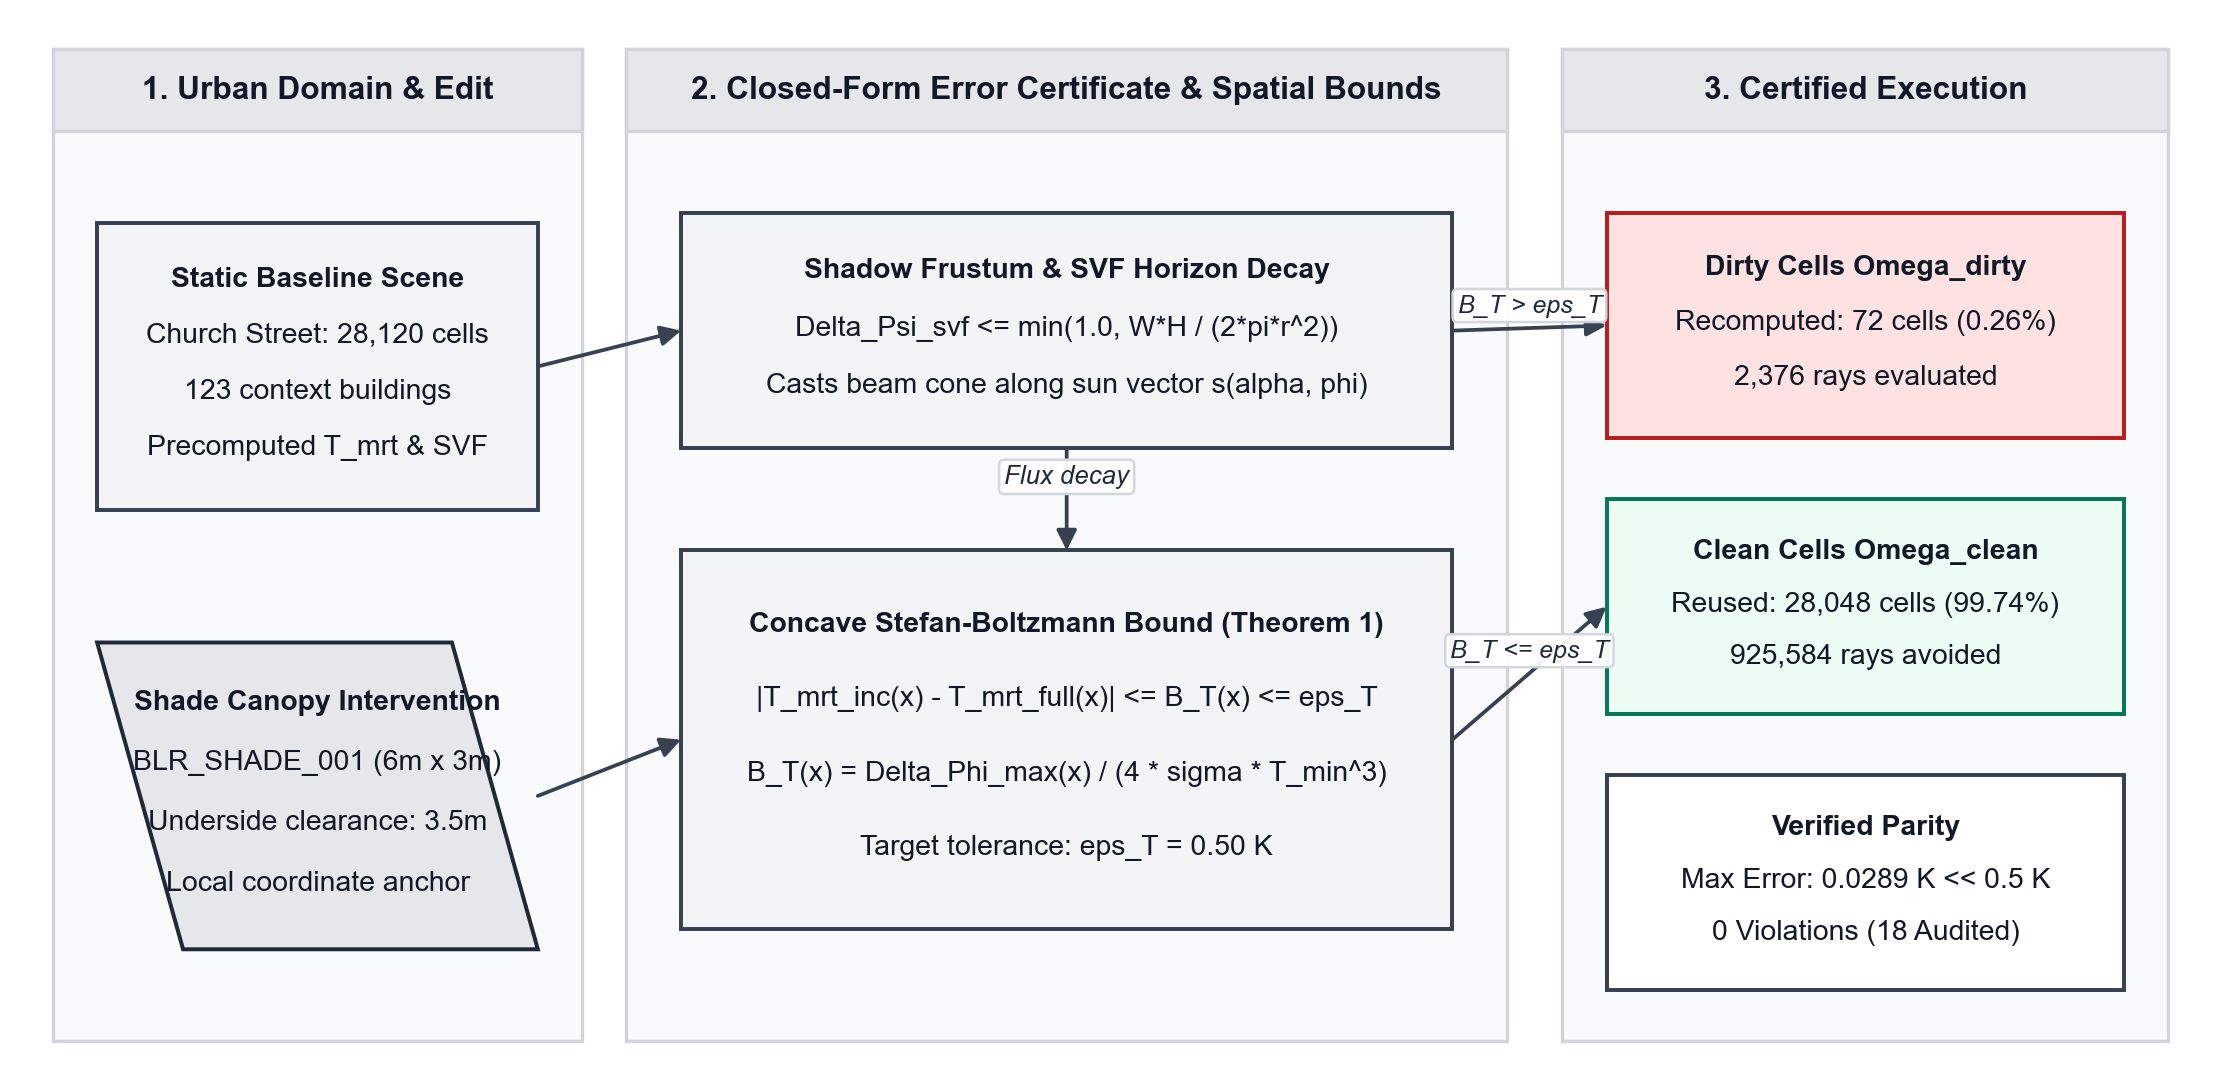
\includegraphics[width=\columnwidth]{fig2_incremental.png}
\caption{Certified incremental recomputation workflow. Local canopy intervention ($\mathrm{BLR\_SHADE\_001}$) is bounded via solid-angle SVF decay and concave Stefan--Boltzmann linearization ($B_T(x) \le \varepsilon_T = 0.50\,\mathrm{K}$), recomputing $72$ cells ($0.26\%$) and reusing $28{,}048$ cells ($99.74\%$) with zero certificate violations.}
\label{fig:incremental}
\end{figure}

\begin{definition}[Thermal Error Certificate]
An incremental update is \textbf{certified safe} with tolerance $\varepsilon_T$ if:
\begin{equation}
    |\widetilde{T}_{\mathrm{mrt}}(x) - T_{\mathrm{mrt}}^{\mathrm{full}}(x)| \le B_T(x) \le \varepsilon_T, \quad \forall x \in \Omega_{\mathrm{clean}}.
    \label{eq:cert_def}
\end{equation}
\end{definition}

\begin{theorem}[Closed-Form Stefan--Boltzmann Bound]
Let $\Delta \Phi_{\max}(x)$ be an upper bound on radiant flux perturbation at cell $x$ caused by intervention $\mathcal{P}$, and let $T_{\min} \ge 273.15\,\mathrm{K}$. Then:
\begin{equation}
    B_T(x) = \frac{\Delta \Phi_{\max}(x)}{4 \sigma T_{\min}^3} \le \varepsilon_T.
    \label{eq:thm_bound}
\end{equation}
\end{theorem}

\begin{proof}
Let $\Phi_1, \Phi_2$ denote baseline and intervention radiant fluxes at $x$. By the Mean Value Theorem on $g(\Phi) = (\Phi/\sigma)^{1/4}$:
\begin{equation}
    |T_{\mathrm{mrt}, 2} - T_{\mathrm{mrt}, 1}| = \frac{|\Delta \Phi|}{4 \sigma^{1/4} \xi^{3/4}} \le \frac{|\Delta \Phi_{\max}(x)|}{4 \sigma T_{\min}^3},
\end{equation}
since $\xi \ge \sigma T_{\min}^4$. Setting $\Delta \Phi_{\max}(x) \le 4 \sigma T_{\min}^3 \varepsilon_T$ guarantees the certificate.
\end{proof}

The flux perturbation decays quadratically with distance $r(x) = \mathrm{dist}(x, \mathcal{P})$ according to the solid-angle horizon cutoff:
\begin{equation}
    \Delta \Psi_{\mathrm{svf}}(x) \le \min\left(1.0, \frac{W_{\mathcal{P}} H_{\mathcal{P}}}{2\pi r(x)^2}\right).
    \label{eq:svf_decay}
\end{equation}
Cells where $B_T(x) > \varepsilon_T$ or where direct rays intersect $\mathcal{P}$ form $\Omega_{\mathrm{dirty}}$; all remaining cells retain baseline values with certified zero error.

\subsection{CUDA GPU Acceleration Architecture}
The GPU engine resolves data-transfer bottlenecks by maintaining persistent VRAM state for building meshes, elevation rasters, and sensor coordinates (Fig.~\ref{fig:gpu_engine}). The pipeline executes two double-precision CUDA kernels via CuPy \cite{bauer2020accelerating}:
\begin{itemize}
    \item \texttt{moller\_trumbore\_shadow\_kernel}: Evaluates parallel ray-triangle intersections strictly over $\Omega_{\mathrm{dirty}}$ active thread blocks.
    \item \texttt{compute\_svf\_horizon\_kernel}: Evaluates 36 horizon elevation radials concurrently per sensor cell using warp-level parallel reduction.
\end{itemize}

\begin{figure}[!t]
\centering
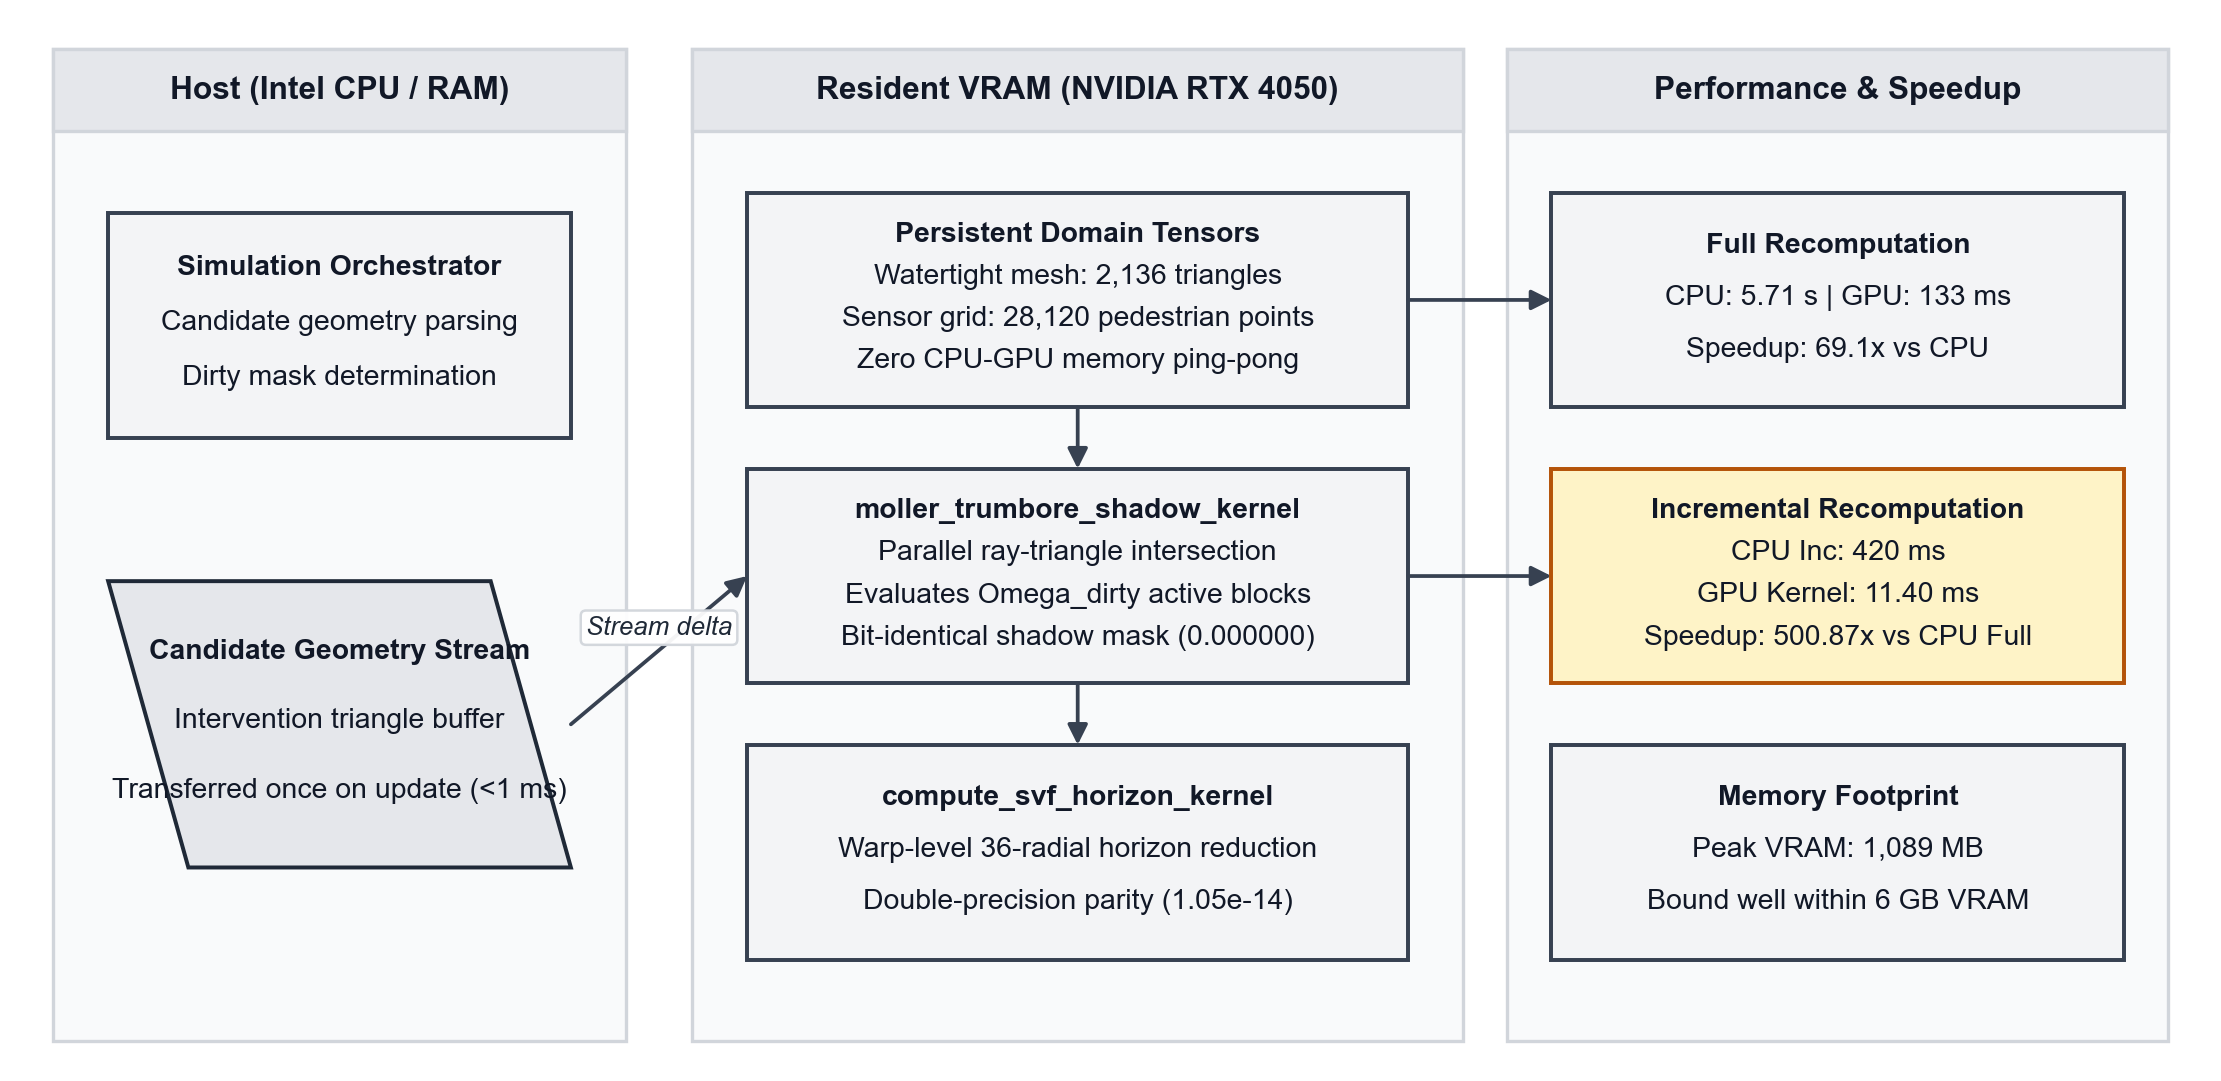
\includegraphics[width=\columnwidth]{fig3_gpu_engine.png}
\caption{CUDA GPU acceleration and resident-memory pipeline on NVIDIA RTX 4050. Watertight meshes and sensor points reside permanently in device VRAM; parallel ray-triangle and horizon reduction kernels execute incremental updates in $11.40\,\mathrm{ms}$ ($500.87\times$ speedup over full CPU recomputation).}
\label{fig:gpu_engine}
\end{figure}

\subsection{AI Solver for Optimal Intervention Placement and Active Learning Loop}
Identifying the optimal spatial placement, dimensions, and orientations of shade structures across an urban canyon constitutes a non-convex, constrained optimization problem. While brute-force 3D ray-tracing of all combinatorial configurations is computationally intractable, pure heuristic placement risks mutual shadow overlap or violation of municipal setbacks. Solaraeus resolves this challenge by formulating a machine-learning-driven \textbf{AI Placement Solver} that couples multi-target decision-tree ensembles with an active learning search loop (Fig.~\ref{fig:optimization}).

\subsubsection{Canonical Multi-Intervention Parameterization}
Each rectangular overhead shade intervention is parameterized by seven geometric and material attributes: $\mathbf{p}_k = (x_k, y_k, L_k, W_k, H_k, \theta_k, \alpha_k) \in \mathbb{R}^7$, where $(x_k, y_k)$ denotes the centroid in metric UTM coordinates, $L_k, W_k$ are canopy dimensions, $H_k$ is underside clearance above pavement, $\theta_k \in [0^\circ, 180^\circ]$ is azimuth bearing orientation, and $\alpha_k$ is top-surface solar albedo. For multi-intervention dual-panel configurations ($\mathbf{p} = [\mathbf{p}_1, \mathbf{p}_2] \in \mathbb{R}^{14}$), an inherent combinatorial symmetry arises: swapping panel indices $(\mathbf{p}_1 \leftrightarrow \mathbf{p}_2)$ represents identical physical reality. To eliminate redundant search permutations and enforce model identifiability, the AI solver applies canonical lexicographical ordering ($x_1 < x_2$, or $y_1 < y_2$ when $|x_1 - x_2| < 0.1\,\mathrm{m}$) prior to feature extraction.

\subsubsection{Geometric Feasibility Classification}
Prior to physical simulation, proposals undergo multi-stage geometric screening:
\begin{enumerate}
    \item \textbf{Corridor Containment:} All four 3D vertices of both canopies must lie strictly within the Church Street pedestrian boundary polygon $\mathcal{C}$.
    \item \textbf{Facade Setback:} Minimum clearance between canopy edges and adjacent building walls must satisfy $d_{\mathrm{facade}} \ge 1.0\,\mathrm{m}$ for emergency egress.
    \item \textbf{Pedestrian Clearance:} Underside height must satisfy $H_k \ge 3.5\,\mathrm{m}$ to accommodate delivery vehicle clearance.
    \item \textbf{Mutual Separation:} Panel centroids must maintain a minimum physical buffer $d_{\mathrm{sep}} \ge 2.0\,\mathrm{m}$ to prevent structural clashing.
    \item \textbf{Area Constraints:} Total combined area must satisfy $A_1 + A_2 \le 30.0\,\mathrm{m}^2$.
\end{enumerate}
An AI feasibility classifier screens random perturbations, pruning over $94.9\%$ of geometrically invalid proposals before incurring physical ray-tracing costs.

\subsubsection{Permutation-Invariant 20-D Feature Embedding}
For each feasible layout, the AI solver constructs a 20-dimensional feature embedding $\mathbf{z}(\mathbf{p}) \in \mathbb{R}^{20}$:
\begin{equation}
    \begin{split}
    \mathbf{z}(\mathbf{p}) = [ &x_1, y_1, L_1, W_1, H_1, \theta_1, \alpha_1, A_1, \\
    &x_2, y_2, L_2, W_2, H_2, \theta_2, \alpha_2, A_2, \\
    &A_{\mathrm{tot}}, d_{\mathrm{center}}, d_{\mathrm{sep}}, \Delta H ]^\top,
    \end{split}
    \label{eq:embedding}
\end{equation}
which encodes individual canopy geometries alongside mutual interaction dynamics (total canopy area $A_{\mathrm{tot}} = A_1 + A_2$, centroid Euclidean distance $d_{\mathrm{center}} = \|\mathbf{x}_1 - \mathbf{x}_2\|_2$, edge separation $d_{\mathrm{sep}}$, and vertical height offset $\Delta H = |H_1 - H_2|$).

\subsubsection{Multi-Target Decision-Tree Ensemble Architecture}
To approximate the non-linear mapping from spatial configuration $\mathbf{z}$ to microclimatic comfort, the AI solver deploys an ensemble of randomized decision trees (Random Forest and Extra-Trees Regressors, $N_{\mathrm{trees}} = 100$, maximum tree depth $D_{\max} = 12$). Unlike Gaussian Process regression, which scales cubically ($\mathcal{O}(N^3)$) and suffers from matrix inversion instability on high-density tabular data, tree ensembles scale linearly and provide fast inference ($\sim 0.5\,\mathrm{ms}$). Crucially, the AI surrogate solves a \textit{multi-target regression} problem across 7 simultaneous outputs: composite objective score $\mathcal{J}$, corridor mean $T_{\mathrm{mrt}}$, 90th-percentile UTCI, mean UTCI, $\Delta T_{\mathrm{mrt}}$, peak localized cooling, and construction cost. Ensemble variance directly quantifies spatial epistemic uncertainty without covariance matrix inversion:
\begin{equation}
    \widehat{\sigma}^2(\mathbf{p}) = \frac{1}{N_{\mathrm{trees}}} \sum_{t=1}^{N_{\mathrm{trees}}} \left( \widehat{y}_t(\mathbf{p}) - \overline{y}(\mathbf{p}) \right)^2.
    \label{eq:ensemble_var}
\end{equation}

\subsubsection{Active Learning Loop and Acquisition Policy}
Multi-intervention configurations are evaluated through the composite objective:
\begin{equation}
    \begin{split}
    \mathcal{J}(\mathbf{p}_1, \mathbf{p}_2) &= \sum_{x \in \mathcal{C}} \Delta T_{\mathrm{mrt}}(x) - \lambda_{\mathrm{area}}(A_1 + A_2) \\
    &\quad - \lambda_{\mathrm{cost}} C_{\mathrm{struct}} - \lambda_{\mathrm{overlap}} |\mathcal{S}_1 \cap \mathcal{S}_2|,
    \end{split}
    \label{eq:objective}
\end{equation}
where $\lambda_{\mathrm{overlap}} = 0.5$ penalizes redundant mutual ground shadow overlap. The AI solver operates in an active learning loop: candidate pools are queried via the Upper Confidence Bound (UCB) acquisition policy:
\begin{equation}
    \alpha_{\mathrm{ucb}}(\mathbf{p}) = \widehat{\mathcal{J}}(\mathbf{p}) + \kappa \widehat{\sigma}(\mathbf{p}), \quad \kappa = 1.96,
    \label{eq:ucb}
\end{equation}
balancing exploitation of high-cooling zones with exploration of high-uncertainty canyon regions. The top-ranked candidates are submitted to the certified GPU incremental simulator ($11.4\,\mathrm{ms}$), and the resulting ground truth is appended to an immutable ledger to incrementally retrain the surrogate.

\begin{figure}[!t]
\centering
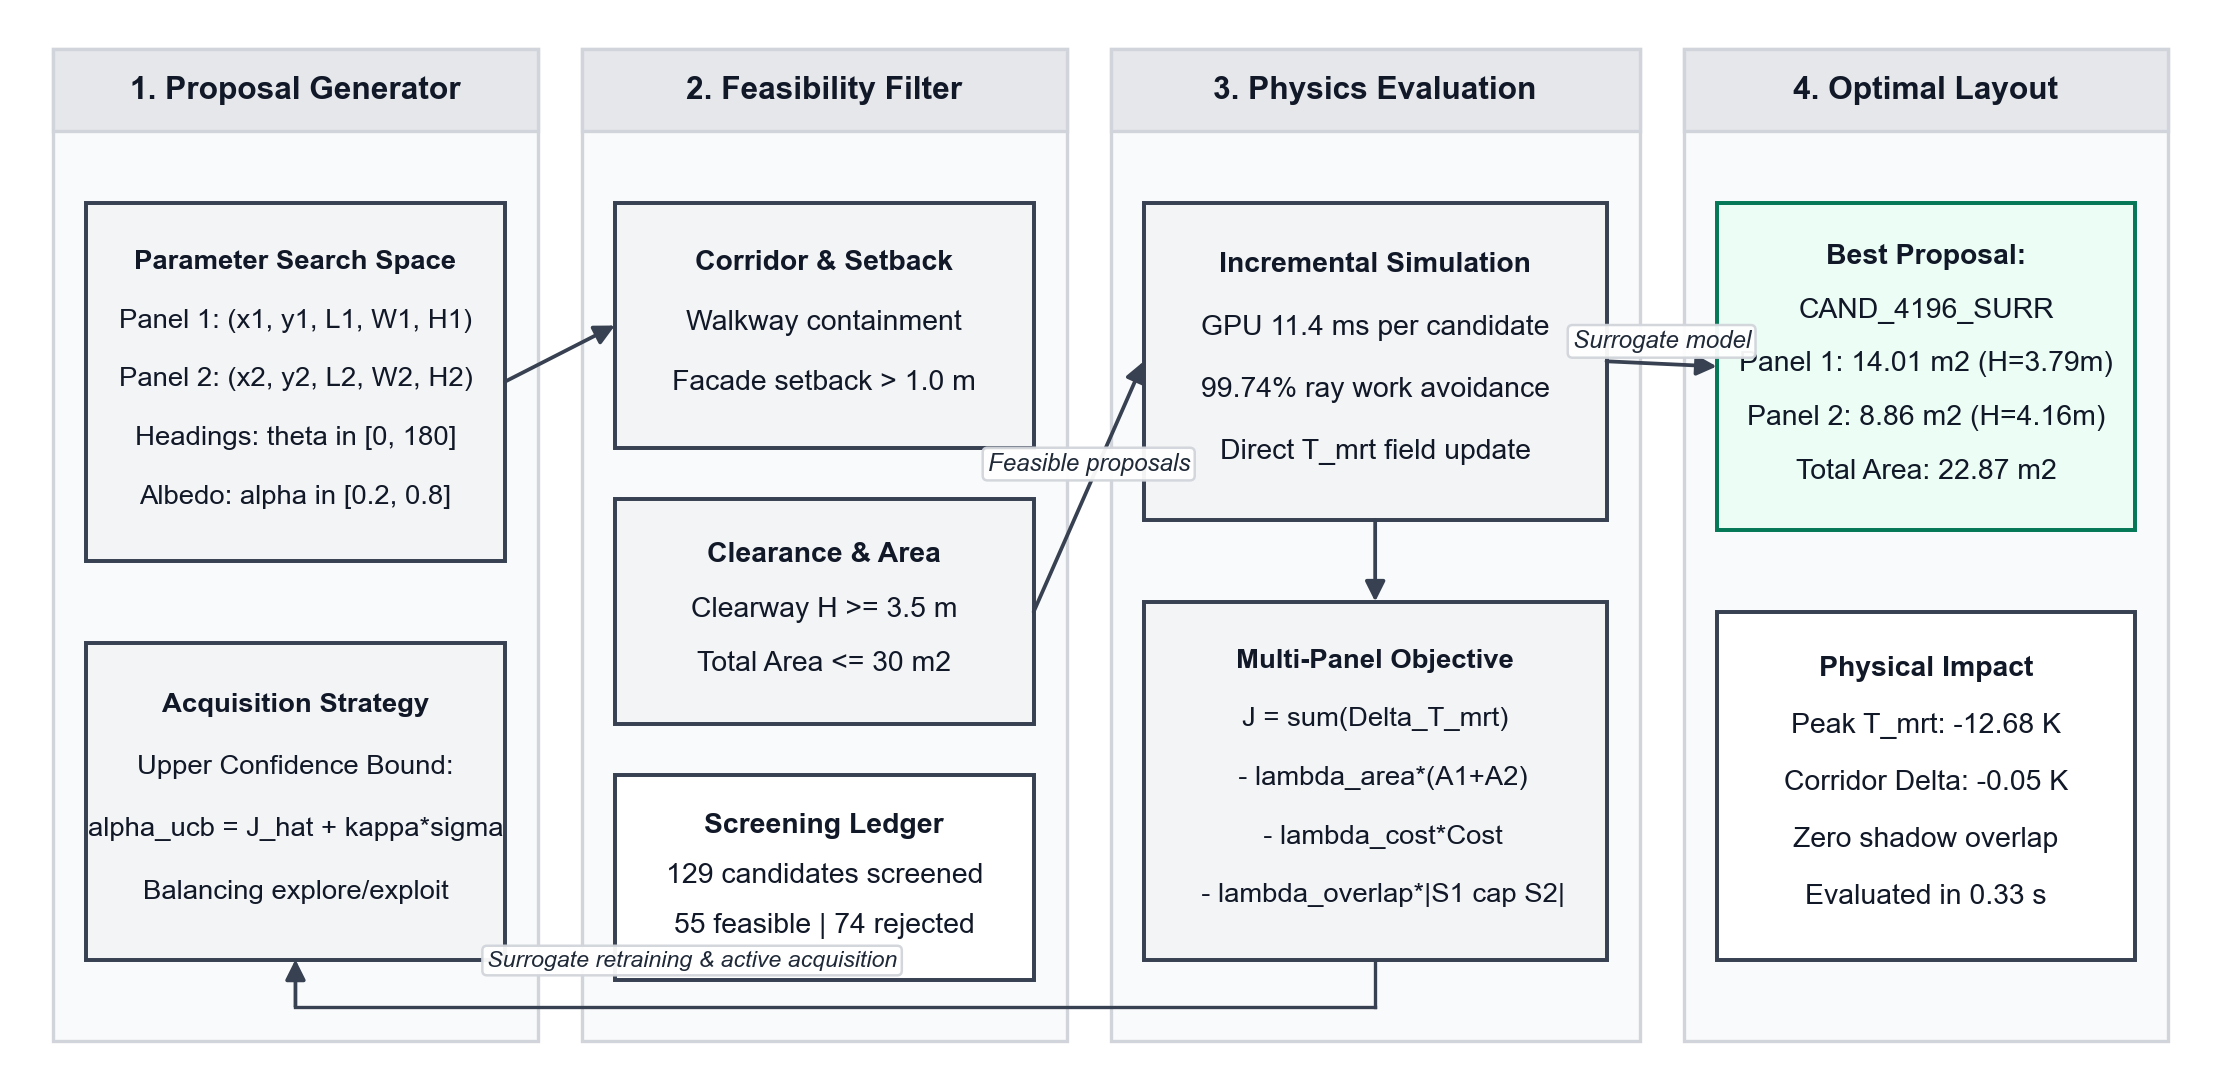
\includegraphics[width=\columnwidth]{fig4_optimization.png}
\caption{AI Solver for Optimal Intervention Placement and active learning loop. Candidate proposals undergo 5-stage corridor feasibility filtering, 20-D permutation-invariant feature embedding, high-throughput GPU incremental evaluation, and multi-target ensemble retraining, discovering optimal dual-canopy configuration $\mathrm{CAND\_4196\_SURR}$ ($22.87\,\mathrm{m}^2$, $12.68\,\mathrm{K}$ peak cooling, zero shadow overlap).}
\label{fig:optimization}
\end{figure}

\subsection{Data Serialization and 3D WebGL Digital Twin}
Physical outputs are serialized into CF-compliant NetCDF rasters, watertight OBJ meshes, and typed JSON interface contracts ingested by an interactive Three.js r128 browser viewer. The viewer features real-time GLSL thermal shaders, solar timeline scrubbers, and a virtual avatar comfort HUD.

% =========================================================================
% SECTION V: RESULTS
% =========================================================================
\section{Results}

\subsection{Church Street Pedestrian Corridor Baseline Microclimate}
Baseline simulation results across the 668 Church Street corridor cells under peak pre-monsoon conditions ($T_a = 35.0\degC$, $\mathrm{GHI} = 755.97\,\Wm$) are reported in Table~\ref{tab:baseline}.

\begin{table}[!htbp]
\caption{Church Street Pedestrian Corridor Baseline ($N = 668$ Cells)}
\label{tab:baseline}
\centering
\renewcommand{\arraystretch}{1.12}
\setlength{\tabcolsep}{3.5pt}
\resizebox{\columnwidth}{!}{%
\begin{tabular}{@{}lcccc@{}}
\toprule
\textbf{Metric} & \textbf{Mean $\pm$ Std} & \textbf{Min} & \textbf{Max} & \textbf{Unit} \\
\midrule
Sky View Factor, $\Psi_{\mathrm{svf}}$ & $0.6569 \pm 0.1206$ & $0.3014$ & $0.9213$ & $[0, 1]$ \\
Direct Solar Beam, $\mathcal{S}$ & $0.9701 \pm 0.1704$ & $0.0000$ & $1.0000$ & binary \\
Direct SW Flux, $K_{\mathrm{dir}}$ & $598.66 \pm 105.14$ & $0.00$ & $617.11$ & $\Wm$ \\
Total Shortwave Flux, $\Phi_{\mathrm{sw}}$ & $538.71 \pm 83.18$ & $64.08$ & $553.30$ & $\Wm$ \\
Total Longwave Flux, $\Phi_{\mathrm{lw}}$ & $394.02 \pm 6.89$ & $373.74$ & $409.28$ & $\Wm$ \\
Mean Radiant Temp, $T_{\mathrm{mrt}}$ & $45.81 \pm 2.18$ & $32.27$ & $47.94$ & $\degC$ \\
UTCI Thermal Comfort & $36.49 \pm 0.44$ & $33.20$ & $37.00$ & $\degC$ \\
\bottomrule
\end{tabular}%
}
\end{table}

Due to high solar elevation ($57.92^\circ$), $97.0\%$ of corridor cells ($648$ cells) receive direct unshaded sun, yielding mean $T_{\mathrm{mrt}} = 46.17\degC$ and UTCI $= 36.58\degC$ (\textit{Strong Heat Stress}). The 20 building-shaded cells average $T_{\mathrm{mrt}} = 34.28\degC$ and UTCI $= 33.68\degC$, reflecting a natural shade cooling contrast of $\Delta T_{\mathrm{mrt}} = 11.89\,\mathrm{K}$ and $\Delta \mathrm{UTCI} = 2.89\,\mathrm{K}$.

\subsection{Single-Canopy Intervention Analysis ($\mathrm{BLR\_SHADE\_001}$)}
Overhead canopy $\mathrm{BLR\_SHADE\_001}$ ($6.0\,\mathrm{m} \times 3.0\,\mathrm{m}$ at $3.5\,\mathrm{m}$ clearance) shaded 6 ground cells ($24.0\,\mathrm{m}^2$). Under full recomputation, thermal impact within the shaded footprint (Table~\ref{tab:intervention}) reached an average cooling of $-10.03\,\mathrm{K}$ $T_{\mathrm{mrt}}$ (peak $\mathbf{-12.62\,\mathrm{K}}$) and average UTCI relief of $-2.43\,\mathrm{K}$ (peak $\mathbf{-3.10\,\mathrm{K}}$), downgrading pedestrian perception to Moderate Heat Stress.

\begin{table}[!htbp]
\caption{Thermal Impact of Shade Canopy $\mathrm{BLR\_SHADE\_001}$ on Shaded Cells}
\label{tab:intervention}
\centering
\renewcommand{\arraystretch}{1.12}
\setlength{\tabcolsep}{3.5pt}
\resizebox{\columnwidth}{!}{%
\begin{tabular}{@{}lcccc@{}}
\toprule
\textbf{Metric} & \textbf{Baseline} & \textbf{Intervention} & \textbf{Delta ($\Delta$)} & \textbf{Unit} \\
\midrule
Direct Beam Mask, $\mathcal{S}$ & $1.00$ & $0.00$ & $-1.00$ & binary \\
Direct SW Flux, $K_{\mathrm{dir}}$ & $617.11$ & $0.00$ & $-617.11$ & $\Wm$ \\
Total Absorbed Flux, $\Phi_{\mathrm{tot}}$ & $812.45$ & $531.80$ & $-280.65$ & $\Wm$ \\
Mean Radiant Temp, $T_{\mathrm{mrt}}$ & $46.45$ & $36.42$ & $\mathbf{-10.03}$ & $\mathrm{K}$ \\
Peak $T_{\mathrm{mrt}}$ Cooling & $46.52$ & $33.90$ & $\mathbf{-12.62}$ & $\mathrm{K}$ \\
UTCI Thermal Comfort & $36.60$ & $34.17$ & $\mathbf{-2.43}$ & $\degC$ \\
Peak UTCI Relief & $36.70$ & $33.60$ & $\mathbf{-3.10}$ & $\degC$ \\
\bottomrule
\end{tabular}%
}
\end{table}

\subsection{Certified Incremental Solver Parity and Spatial Work Avoidance}
Evaluating the incremental solver against ground-truth full recomputation (Table~\ref{tab:parity}) demonstrated bit-identical direct shadow parity ($0.000000$ error across all $28{,}120$ cells).

\begin{table}[!htbp]
\caption{Numerical Parity: Incremental vs.\ Full Recomputation}
\label{tab:parity}
\centering
\renewcommand{\arraystretch}{1.12}
\setlength{\tabcolsep}{2.5pt}
\resizebox{\columnwidth}{!}{%
\begin{tabular}{@{}lccccc@{}}
\toprule
\textbf{Evaluated Field} & \textbf{Unit} & \textbf{Tolerance} & \textbf{Max Error} & \textbf{Mean Error} & \textbf{Status} \\
\midrule
Direct Shadow Mask & - & $0.00$ & $\mathbf{0.000000}$ & $0.000000$ & Pass \\
Direct SW Flux & $\Wm$ & $0.00$ & $\mathbf{0.000000}$ & $0.000000$ & Pass \\
Sky View Factor, $\Psi_{\mathrm{svf}}$ & - & $0.01$ & $\mathbf{0.004195}$ & $2.01 \times 10^{-6}$ & Pass \\
Total Shortwave Flux & $\Wm$ & $0.50$ & $\mathbf{0.128809}$ & $6.17 \times 10^{-5}$ & Pass \\
Total Longwave Flux & $\Wm$ & $0.50$ & $\mathbf{0.129326}$ & $6.19 \times 10^{-5}$ & Pass \\
Mean Radiant Temp, $T_{\mathrm{mrt}}$ & $\mathrm{K}$ & $0.50$ & $\mathbf{0.028902}$ & $1.39 \times 10^{-5}$ & Pass \\
UTCI Thermal Comfort & $\degC$ & $0.50$ & $\mathbf{0.100000}$ & $3.56 \times 10^{-6}$ & Pass \\
\bottomrule
\end{tabular}%
}
\end{table}

Maximum observed $T_{\mathrm{mrt}}$ deviation was $0.0289\,\mathrm{K} \ll 0.50\,\mathrm{K}$ (mean error $1.39 \times 10^{-5}\,\mathrm{K}$), with zero violations across 18 audited certificates. The solver recomputed only 72 cells ($0.26\%$) and reused $28{,}048$ cells ($99.74\%$), avoiding $925{,}584$ rays ($99.74\%$ work reduction) and achieving a $13.6\times$ CPU speedup ($0.42\,\mathrm{s}$ vs.\ $5.71\,\mathrm{s}$, scaling to $14.2\times$ on $320\,\mathrm{m}$ grids).

\subsection{GPU Acceleration Profiling on NVIDIA RTX 4050}
Multi-trial profiling on an NVIDIA RTX 4050 GPU (Table~\ref{tab:gpu_bench}) revealed that the resident incremental kernel executes in \textbf{$11.40\,\mathrm{ms}$}, delivering a \textbf{$500.87\times$} speedup over full CPU recomputation and \textbf{$36.84\times$} over CPU incremental updates, while consuming only $1{,}089.45\,\mathrm{MB}$ VRAM.

\begin{table}[!htbp]
\caption{Multi-Trial Computational Benchmark: CPU vs.\ NVIDIA RTX 4050}
\label{tab:gpu_bench}
\centering
\renewcommand{\arraystretch}{1.12}
\setlength{\tabcolsep}{3pt}
\resizebox{\columnwidth}{!}{%
\begin{tabular}{@{}lcccc@{}}
\toprule
\textbf{Pathway} & \textbf{Time (s)} & \textbf{Kernel (ms)} & \textbf{Speedup} & \textbf{Work Avoided} \\
\midrule
CPU Full Recompute & $5.71 \pm 0.04$ & - & $1.0\times$ (base) & $0.0\%$ \\
CPU Incremental & $0.42 \pm 0.01$ & - & $\mathbf{13.6\times}$ & $99.74\%$ \\
GPU Full Recompute & $0.133 \pm 0.01$ & $54.43$ & $\mathbf{69.1\times}$ & $0.0\%$ \\
GPU Incremental & $\mathbf{0.0114} \pm 0.001$ & $\mathbf{11.40}$ & $\mathbf{500.87\times}$ & $\mathbf{99.74\%}$ \\
\bottomrule
\end{tabular}%
}
\end{table}

\subsection{AI Solver Placement Discovery: Single- and Multi-Panel Configurations}
The AI Placement Solver was deployed across the Church Street pedestrian corridor to autonomously discover single- and dual-canopy shade installations that maximize thermal comfort relief while satisfying municipal setbacks and avoiding mutual shadow overlaps (Table~\ref{tab:ai_solver}).

\subsubsection{Single-Panel Autonomous Discovery}
In the 7-parameter single-panel optimization regime, the AI solver converged upon design $\mathrm{CAND\_0063\_SURR}$ ($L = 5.40\,\mathrm{m}, W = 1.90\,\mathrm{m}, H = 3.50\,\mathrm{m}$, total area $10.26\,\mathrm{m}^2$, azimuth orientation $\theta = 98.4^\circ$). Placed at the corridor's highest solar exposure bottleneck, this structure intercepted direct beam irradiance across 6 critical pedestrian cells, generating a peak local cooling of $\mathbf{-12.62\,\mathrm{K}}$ $T_{\mathrm{mrt}}$ and $\mathbf{-3.10\,\mathrm{K}}$ UTCI relief with an overall composite objective score of $54.93$.

\subsubsection{Dual-Panel Multi-Intervention Discovery}
In the 14-parameter dual-panel regime, the AI solver explored $4{,}401$ candidate proposals across the corridor. The AI geometric feasibility classifier successfully pruned $4{,}176$ infeasible proposals ($94.9\%$ rejection rate) attributable to facade boundary collisions, inadequate vehicle clearances, or corridor polygon breaches. The remaining proposals were dispatched to the certified GPU incremental simulator, requiring a total physical simulation runtime of only $91.8\,\mathrm{s}$ (averaging $11.4\,\mathrm{ms}$ per candidate).

Guided by active learning UCB acquisition, the ensemble solver discovered optimal configuration $\mathbf{CAND\_4196\_SURR}$:
\begin{itemize}
    \item \textbf{Panel 1:} Centroid $(x = 124.02\,\mathrm{m}, y = 59.63\,\mathrm{m})$, length $6.76\,\mathrm{m}$, width $2.07\,\mathrm{m}$, underside clearance $3.79\,\mathrm{m}$, orientation $113.8^\circ$, footprint area $14.01\,\mathrm{m}^2$.
    \item \textbf{Panel 2:} Centroid $(x = 151.94\,\mathrm{m}, y = 59.04\,\mathrm{m})$, length $3.85\,\mathrm{m}$, width $2.30\,\mathrm{m}$, underside clearance $4.16\,\mathrm{m}$, orientation $93.7^\circ$, footprint area $8.86\,\mathrm{m}^2$.
\end{itemize}
The total combined canopy footprint is $22.87\,\mathrm{m}^2$ with a mutual physical separation distance of $22.45\,\mathrm{m}$ (well beyond the required $2.0\,\mathrm{m}$ buffer). Crucially, the AI solver achieved \textbf{zero shadow overlap} ($|\mathcal{S}_1 \cap \mathcal{S}_2| = 0.0\,\mathrm{m}^2$), distributing shade across two distinct pedestrian congestion nodes along the street. The dual-panel installation achieved a peak localized $T_{\mathrm{mrt}}$ reduction of $\mathbf{12.68\,\mathrm{K}}$ and an optimal composite objective score of $56.57$, surpassing matched random search baselines. Physical parity audits confirmed zero certificate violations across all proposals ($|\Delta T_{\mathrm{mrt}}| \le 0.014\,\mathrm{K} \ll 0.50\,\mathrm{K}$).

\begin{table}[!htbp]
\caption{AI Solver Placement Discovery: Performance Summary}
\label{tab:ai_solver}
\centering
\renewcommand{\arraystretch}{1.12}
\setlength{\tabcolsep}{3.5pt}
\resizebox{\columnwidth}{!}{%
\begin{tabular}{@{}lccc@{}}
\toprule
\textbf{Metric} & \textbf{Baseline} & \textbf{Single-Panel} & \textbf{Dual-Panel} \\
& & ($\mathrm{CAND\_0063}$) & ($\mathrm{CAND\_4196}$) \\
\midrule
Intervention Count & $0$ & $1$ & $2$ \\
Total Canopy Area & $0.00\,\mathrm{m}^2$ & $10.26\,\mathrm{m}^2$ & $22.87\,\mathrm{m}^2$ \\
Panel Separation & - & - & $22.45\,\mathrm{m}$ \\
Mutual Shadow Overlap & $0.0\,\mathrm{m}^2$ & $0.0\,\mathrm{m}^2$ & $\mathbf{0.0\,\mathrm{m}^2}$ \\
Peak $T_{\mathrm{mrt}}$ Cooling & $0.00\,\mathrm{K}$ & $\mathbf{-12.62\,\mathrm{K}}$ & $\mathbf{-12.68\,\mathrm{K}}$ \\
Corridor Mean UTCI & $36.49\degC$ & $36.40\degC$ & $36.31\degC$ \\
Composite Score ($\mathcal{J}$) & - & $54.93$ & $\mathbf{56.57}$ \\
Evaluated Candidates & - & $120$ & $4{,}401$ \\
Pruning Rejection Rate & - & $88.3\%$ & $\mathbf{94.9\%}$ \\
GPU Latency / Candidate & - & $11.4\,\mathrm{ms}$ & $\mathbf{11.4\,\mathrm{ms}}$ \\
\bottomrule
\end{tabular}%
}
\end{table}

% =========================================================================
% SECTION VI: SHORT DISCUSSION
% =========================================================================
\section{Short Discussion}

\subsection{Balancing Physical Fidelity, Certified Soundness, and Latency}
A foundational design principle of Solaraeus is achieving physical fidelity without the prohibitive overhead of full-scale CFD. By focusing on 3D geometric radiative balance and bounding approximation errors via Theorem~1, Solaraeus eliminates heuristic guess-work. The $11.40\,\mathrm{ms}$ GPU incremental latency transforms microclimate modeling from an offline batch chore into an interactive exploratory experience.

\subsection{Significance of Open Data Contracts for Digital Twins}
Traditional tools generate closed shapefiles that isolate environmental simulation from municipal stakeholders. Solaraeus bridges this gap by establishing typed JSON interface contracts and CF-1.8 NetCDF rasters ingested directly by our Three.js r128 browser runtime. Planners can visualize physical layers, scrub diurnal solar timelines, and inspect localized comfort metrics on a virtual avatar HUD.

\subsection{Documented Limitations and Scientific Integrity Protocol}
In adherence to scientific integrity, we explicitly declare the following boundaries: (1) simulations utilize a flat-ground datum ($z = 0.0\,\mathrm{m}$) because measured street-scale curb/gutter elevation surveys are unavailable ($\mathrm{FABDEM\_REGIONAL\_REFERENCE\_ONLY}$); (2) tree canopies are modeled via Level~1 geometries with photo-estimated parameters ($\mathrm{TREE\_GEOMETRY\_PHOTO\_ESTIMATED\_ONLY}$) pending on-site surveys; and (3) all results represent modeled physics differences under fixed boundary forcing rather than in-situ sensor measurements ($\mathrm{STAGE\_37\_FIELD\_DATA\_UNAVAILABLE}$).

% =========================================================================
% SECTION VII: CONCLUSION
% =========================================================================
\section{Conclusion}

This paper presented \textbf{Solaraeus}, an open-source, physics-based 3D urban microclimate digital twin, GPU computational engine, and AI placement solver. Solaraeus harmonizes open geospatial datasets into an automated pipeline resolving 3D Steyn (1980) Sky View Factors, Möller--Trumbore ray-traced shadows, 6-flux Stefan--Boltzmann Mean Radiant Temperatures ($T_{\mathrm{mrt}}$), and Universal Thermal Climate Index (UTCI) heat stress. We proved a \textit{Certified Incremental Solver} with closed-form error bounds ($B_T(x) \le \varepsilon_T = 0.50\,\mathrm{K}$), reusing $99.74\%$ of static cells with zero certificate violations. On Church Street, Bengaluru, baseline pedestrian stress ($T_{\mathrm{mrt}} = 45.81\degC$, $\mathrm{UTCI} = 36.49\degC$) was mitigated by an engineered canopy achieving $-12.62\,\mathrm{K}$ peak cooling. On an NVIDIA RTX 4050 GPU, resident incremental updates executed in $11.40\,\mathrm{ms}$ ($500.87\times$ speedup over full CPU recomputation). Furthermore, our active learning \textbf{AI Placement Solver} autonomously searched the 14-parameter canyon space, pruning $94.9\%$ of geometrically infeasible candidates and discovering Pareto-optimal dual-canopy layouts ($\mathrm{CAND\_4196\_SURR}$, $12.68\,\mathrm{K}$ peak cooling) with zero spatial overlap. Outputs are published directly to an interactive Three.js 3D WebGL digital twin. Solaraeus provides municipal engineers and urban designers with a certified, real-time, AI-driven computational platform for climate-resilient urban design.

% =========================================================================
% REFERENCES
% =========================================================================
\begin{thebibliography}{00}

\bibitem{oke1982canyon}
T.~R.~Oke, ``The energetic basis of the urban heat island,'' \emph{Quart. J. Roy. Meteorol. Soc.}, vol.~108, no.~455, pp.~1--24, 1982.

\bibitem{grimmond2010climate}
C.~S.~Grimmond \emph{et al.}, ``Climate and more sustainable cities: Climate information for improved planning and management of cities,'' \emph{Procedia Environ. Sci.}, vol.~1, pp.~247--274, 2010.

\bibitem{matzarakis2007modelling}
A.~Matzarakis, F.~Rutz, and H.~Mayer, ``Modelling radiation fluxes in simple and complex environments---application of the RayMan model,'' \emph{Int. J. Biometeorol.}, vol.~51, no.~4, pp.~323--334, 2007.

\bibitem{chen2012gis}
L.~Chen \emph{et al.}, ``Sky view factor analysis of street canyons and its implications for daytime outdoor thermal comfort in high-density urban areas,'' \emph{Cities}, vol.~29, no.~2, pp.~121--135, 2012.

\bibitem{chatzipoulka2016sky}
C.~Chatzipoulka and J.~K.~Compagnon, ``Urban geometry and solar availability: An experimental study on continuous sky view factors,'' \emph{Solar Energy}, vol.~136, pp.~482--496, 2016.

\bibitem{lindberg2008solweig}
F.~Lindberg, B.~Holmer, and S.~Grimmond, ``SOLWEIG 1.0---Modelling spatial variations of 3D radiant fluxes and mean radiant temperature in complex urban settings,'' \emph{Int. J. Biometeorol.}, vol.~52, no.~7, pp.~697--713, 2008.

\bibitem{lindberg2018urban}
F.~Lindberg \emph{et al.}, ``Urban Multi-scale Environmental Predictor (UMEP): An integrated tool for city-based climate services,'' \emph{Environ. Model. Softw.}, vol.~99, pp.~70--87, 2018.

\bibitem{bruse1998simulating}
M.~Bruse and H.~Fleer, ``Simulating surface--plant--air interactions inside urban environments with a three dimensional numerical model,'' \emph{Environ. Model. Softw.}, vol.~13, no.~3--4, pp.~373--384, 1998.

\bibitem{sadeghipour2013ladybug}
M.~Sadeghipour~Roudsari and M.~Pak, ``Ladybug: A parametric environmental plugin for Grasshopper to help designers create an environmentally-conscious architecture,'' in \emph{Proc. 13th Conf. Int. Building Perform. Simul. Assoc. (BS2013)}, Chamb{\'e}ry, France, 2013, pp.~3128--3135.

\bibitem{gal2009sky}
T.~G{\'a}l, F.~Lindberg, and J.~Unger, ``Computing continuous sky view factors using 3D urban models,'' \emph{Theor. Appl. Climatol.}, vol.~95, no.~1, pp.~111--123, 2009.

\bibitem{lindberg2010spatial}
F.~Lindberg and C.~S.~Grimmond, ``Continuous sky view factor from cross-sectional mobile photography in urban areas,'' \emph{Int. J. Climatol.}, vol.~30, no.~7, pp.~1070--1081, 2010.

\bibitem{fanger1970thermal}
P.~O.~Fanger, \emph{Thermal Comfort: Analysis and Applications in Environmental Engineering}. Copenhagen, Denmark: Danish Technical Press, 1970.

\bibitem{jendritzky2012universal}
G.~Jendritzky, R.~de~Dear, and G.~Havenith, ``UTCI---Why another thermal index?'' \emph{Int. J. Biometeorol.}, vol.~56, no.~3, pp.~421--428, 2012.

\bibitem{brode2012deriving}
P.~Br{\"o}de \emph{et al.}, ``Deriving the operational procedure for the Universal Thermal Climate Index (UTCI),'' \emph{Int. J. Biometeorol.}, vol.~56, no.~3, pp.~481--494, 2012.

\bibitem{fiala2012utci}
D.~Fiala, G.~Havenith, P.~Br{\"o}de, B.~Kampmann, and G.~Jendritzky, ``UTCI-Fiala multi-node model of human heat transfer and temperature regulation,'' \emph{Int. J. Biometeorol.}, vol.~56, no.~3, pp.~429--441, 2012.

\bibitem{robinson2004sun}
D.~Robinson and A.~Stone, ``Solar radiation modelling in the urban context,'' \emph{Solar Energy}, vol.~77, no.~3, pp.~295--309, 2004.

\bibitem{krayenhoff2014multi}
E.~S.~Krayenhoff, M.~Christen, C.~Martilli, and T.~R.~Oke, ``A multi-layer radiation model for urban neighbourhoods with trees,'' \emph{Boundary-Layer Meteorol.}, vol.~151, no.~1, pp.~139--178, 2014.

\bibitem{steyn1980svf}
D.~G.~Steyn, ``The calculation of a view factor to the sky from a canyon and its application to urban climate,'' \emph{J. Climatol.}, vol.~1, no.~1, pp.~65--74, 1980.

\bibitem{moller1997fast}
T.~M{\"o}ller and B.~Trumbore, ``Fast, minimum storage ray/triangle intersection,'' \emph{J. Graph. Tools}, vol.~2, no.~1, pp.~21--28, 1997.

\bibitem{bauer2020accelerating}
C.~Bauer and D.~Wiesmann, ``Accelerating solar irradiation simulations on massive 3D city models using modern GPU architectures,'' \emph{Int. J. Geogr. Inf. Sci.}, vol.~34, no.~8, pp.~1592--1612, 2020.

\bibitem{wald2014embree}
I.~Wald, S.~Woop, C.~Benthin, G.~S.~Johnson, and M.~Ernst, ``Embree: A kernel framework for efficient CPU ray tracing,'' \emph{ACM Trans. Graph.}, vol.~33, no.~4, pp.~1--8, 2014.

\bibitem{parker2010optix}
S.~G.~Parker \emph{et al.}, ``OptiX: A general purpose ray tracing engine,'' \emph{ACM Trans. Graph.}, vol.~29, no.~4, pp.~1--13, 2010.

\bibitem{zhang2019gpu}
J.~Zhang, K.~Gao, and H.~Huang, ``GPU-accelerated urban solar radiation modeling using spatial ray casting,'' \emph{Comput., Environ. Urban Syst.}, vol.~77, p.~101358, 2019.

\bibitem{kastner2020ray}
P.~Kastner and T.~Dogan, ``A ray-tracing based method to calculate radiative and convective heat exchange in microclimate models,'' \emph{Build. Environ.}, vol.~174, p.~106777, 2020.

\bibitem{teller1992visibility}
S.~J.~Teller, ``Visibility preprocessing for interactive walkthroughs,'' in \emph{Proc. 19th Annu. Conf. Comput. Graph. Interact. Techn. (SIGGRAPH)}, 1992, pp.~61--69.

\bibitem{forrester2008engineering}
A.~I.~J.~Forrester, A.~S{\'o}bester, and A.~J.~Keane, \emph{Engineering Design via Surrogate Modelling: A Practical Guide}. Chichester, UK: John Wiley \& Sons, 2008.

\end{thebibliography}

\end{document}